% Рисуночки
\section{Конструкторская часть}
\subsection{Описания алгоритмов}

\hspace{1.25cm}
На основании теоретических измышлений были разработаны алгоритмы, реализующие линейный и бинарный поиск в массиве. Блок-схемы этих алгоритмов приведены на рисунках \ref{fig:block_1} (линейный) и \ref{fig:block_2} (бинарный).

\begin{figure}[H]
    \centering
    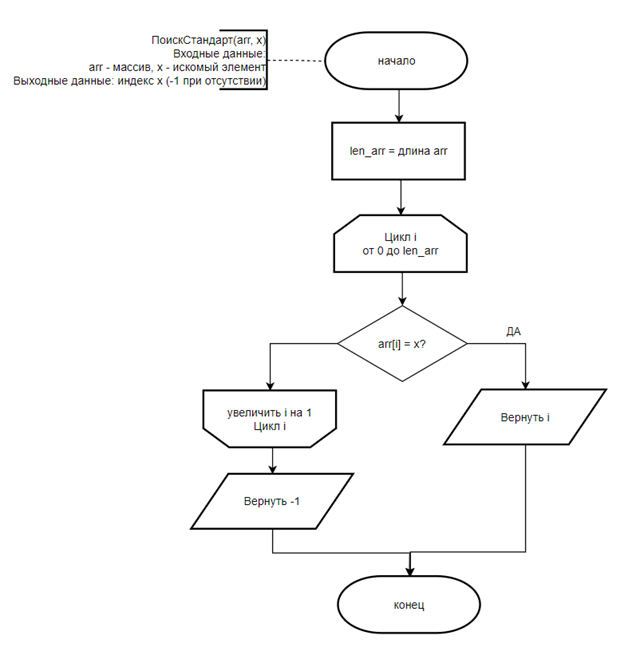
\includegraphics[width=1\textwidth]{img/block_1.png}
    \caption{Блок-схема линейного алгоритма поиска в массиве}
    \label{fig:block_1}
\end{figure}

\begin{figure}[H]
    \centering
    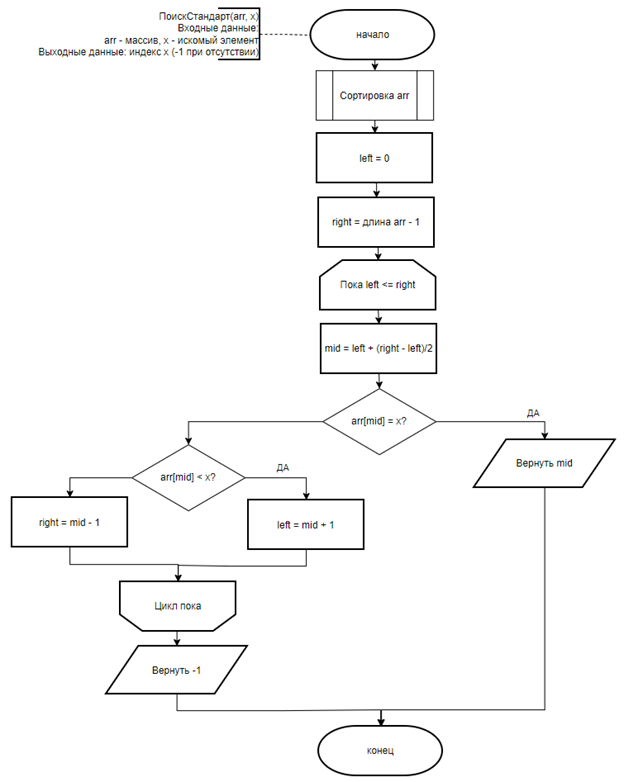
\includegraphics[width=0.9\textwidth]{img/block_2.png}
    \caption{Блок-схема бинарного алгоритма поиска в массиве}
    \label{fig:block_2}
\end{figure}

\newpage